\section{Results and Observations}
\label{sec:results}

The supplied report records PASS outcomes for metainfo, tracker, peer, piece-transfer, multi-torrent, and integration checks. The integrated scenario used two torrents: a 4,099-byte single-file payload and a 3,164-byte multi-file bundle. The total transferred payload was therefore

\begin{equation}
  4{,}099 + 3{,}164 = 7{,}263\ \text{bytes}.
  \label{eq:total-payload}
\end{equation}

The integration assertions require both leecher workers to finish, both seeder workers to remain complete, session upload and download totals to equal 7,263 bytes, and three output files to match their sources. These checks validate the demonstrated workflow but should not be interpreted as a throughput benchmark.

\begin{reportfigure}[0.98\linewidth]{figures/tracker-http-traffic.png}
{Loopback capture of HTTP announce connections between peers and the tracker. File payloads are not present on this tracker connection.}
{fig:tracker-http}
\end{reportfigure}

\begin{reportfigure}[0.98\linewidth]{figures/peer-tcp-traffic.png}
{Loopback capture of direct TCP connections on the configured peer ports.}
{fig:peer-tcp}
\end{reportfigure}

\begin{figure}[tbp]
  \centering
  \begin{subfigure}[t]{0.49\textwidth}
    \centering
    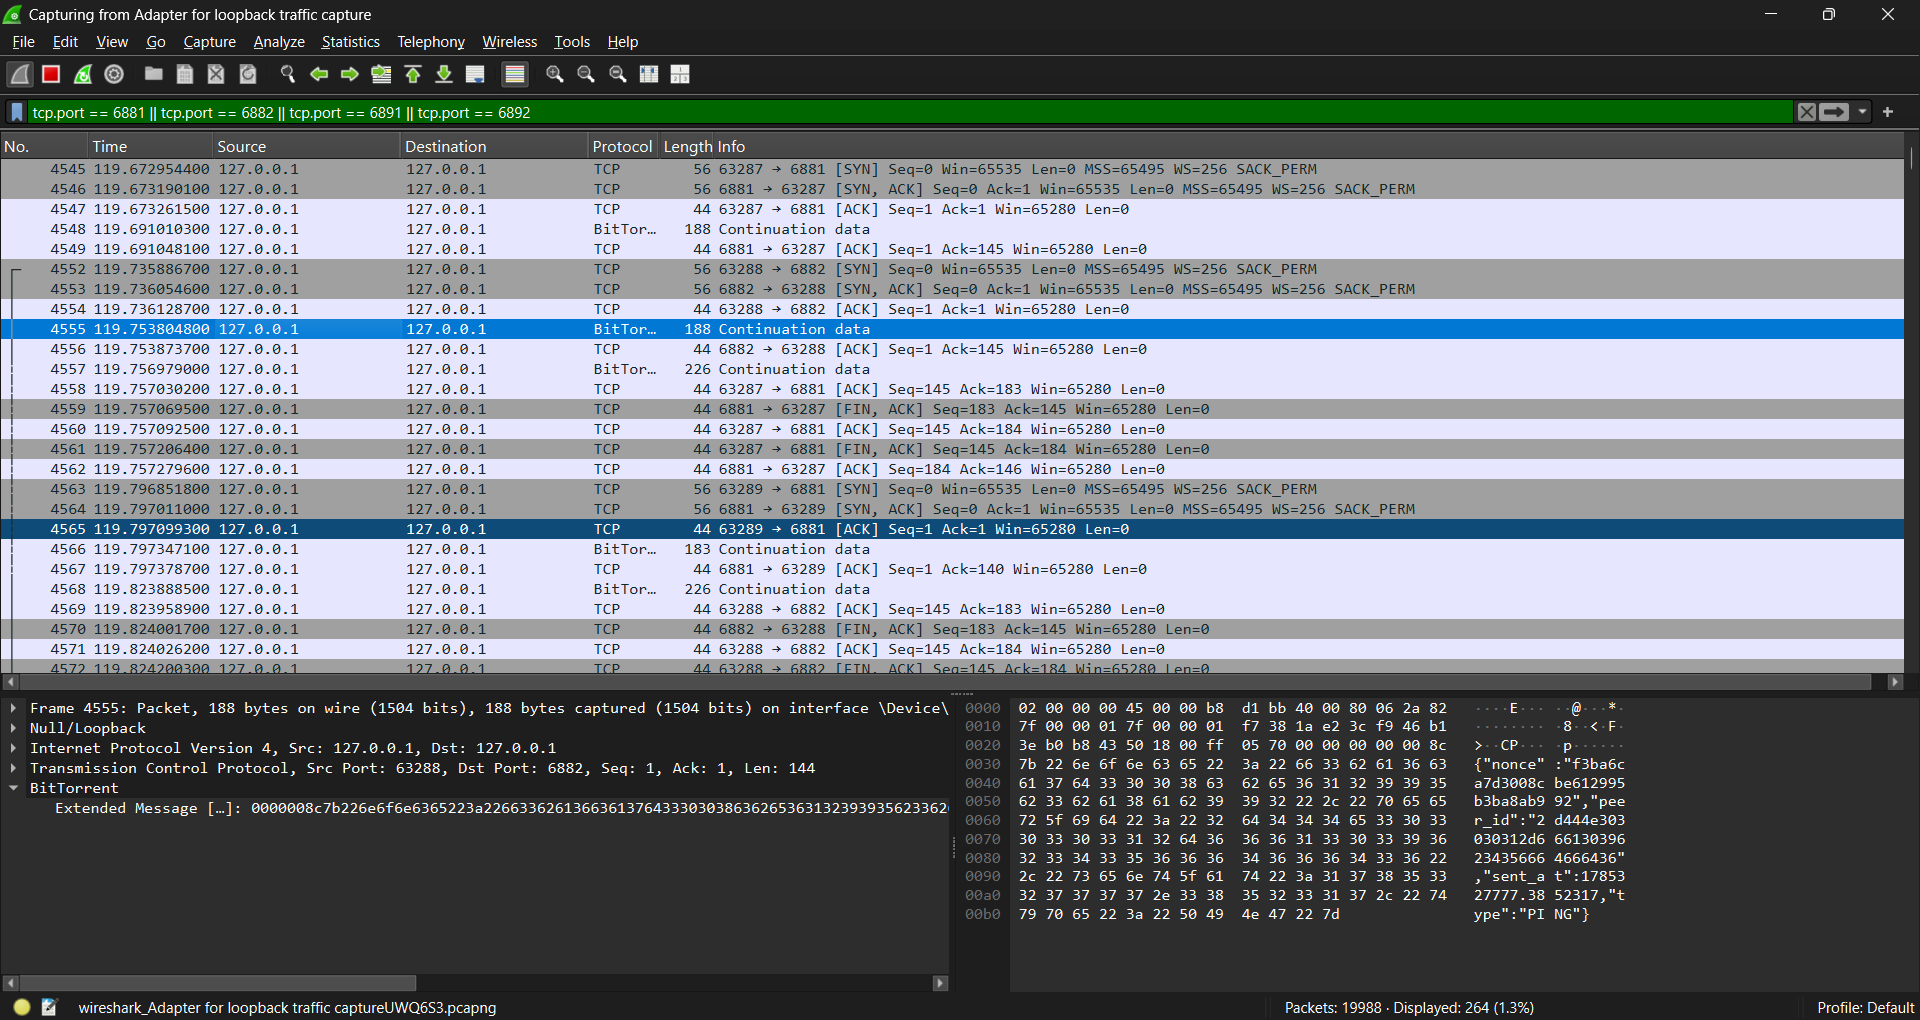
\includegraphics[width=\linewidth]{figures/ping-packet.png}
    \caption{Framed PING message in one peer connection.}
    \label{fig:ping-packet}
  \end{subfigure}\hfill
  \begin{subfigure}[t]{0.49\textwidth}
    \centering
    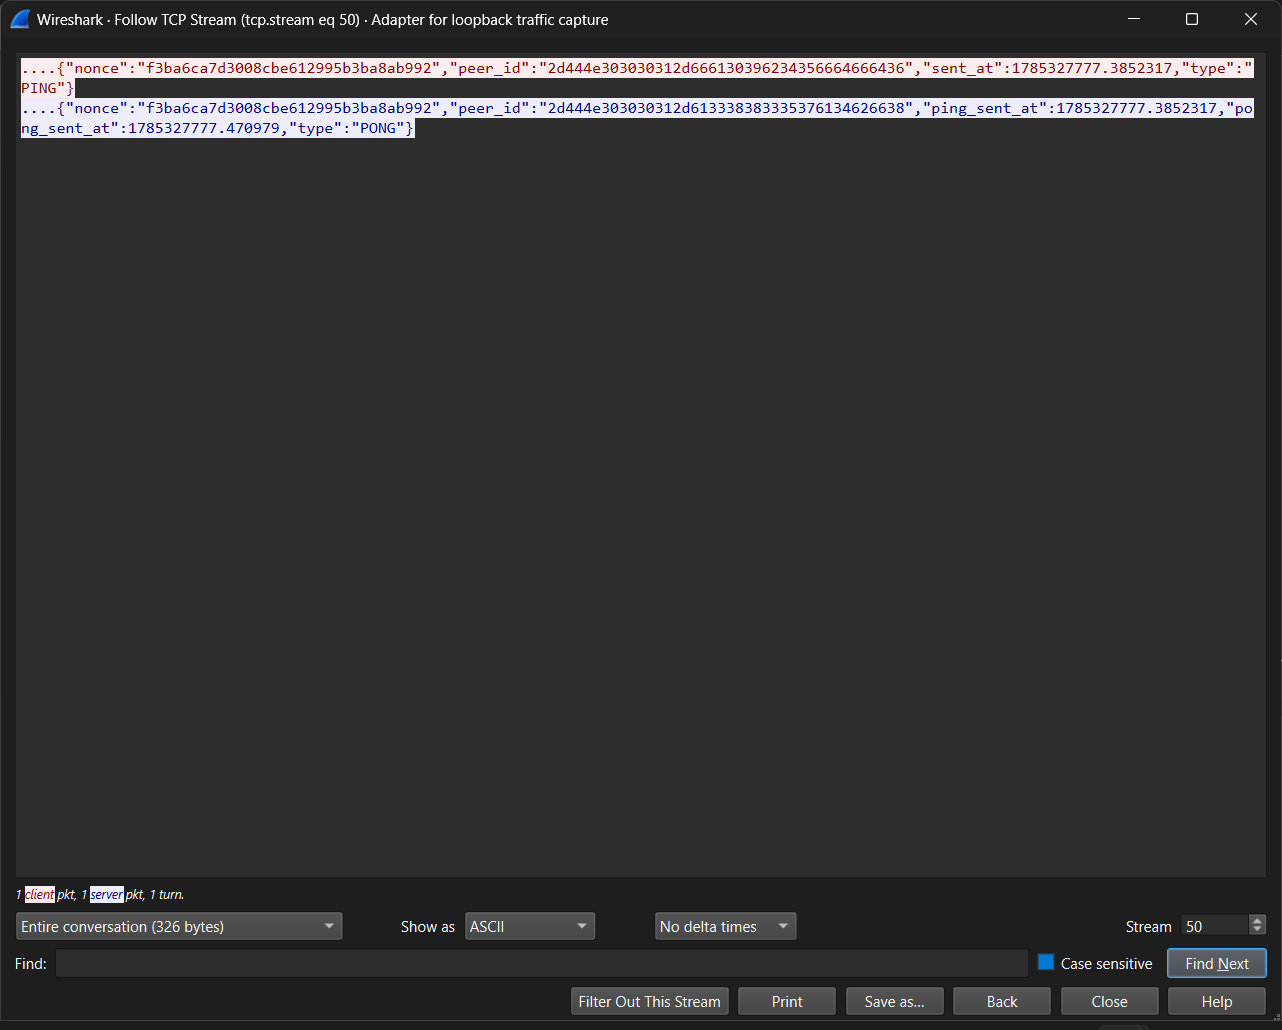
\includegraphics[width=\linewidth]{figures/ping-pong-stream.png}
    \caption{PING and PONG payloads in a followed TCP stream.}
    \label{fig:ping-stream}
  \end{subfigure}
  \caption{Packet-capture evidence for the custom peer reachability exchange.}
  \label{fig:ping-evidence}
\end{figure}

\Cref{fig:tracker-http,fig:peer-tcp} visually separates tracker traffic on port 8000 from direct traffic on peer ports. \Cref{fig:ping-evidence} shows the four-byte frame prefix followed by JSON application data and matching nonce values across PING/PONG. Packet segmentation itself is not used as a correctness criterion; application-level length, piece index, and hash checks provide the relevant validation.
